\section{Applications of Differentiation}

    \subsection{Critical Points}
        $x=c$ is a \textbf{critical point} of the function $f'(x)$ if $f(c)$ exists and \\

        \begin{center}
            \begin{tabular}{ccc}
                $f'(c) = 0$ & OR & $f'(c)$ doesn't exist
            \end{tabular}
        \end{center}

        \noindent \color{blue} \textit{Example: Determine all the critical points for the function} \\

        \begin{equation*}
            f(x) = 6x - 4\cos{(3x)}
        \end{equation*} \color{black} \\

        \begin{align*}
            f'(x) = 0 &= 6 + 12\sin{(3x)} \\
            \sin{(3x)} &= -\frac{1}{2} \\
            x &= 1.2217+\frac{2\pi n}{3}, n=0,\pm 1,\pm 2,\dots \\
            \text{and} \\
            x &= 1.9199+\frac{2\pi n}{3}, n=0,\pm 1,\pm 2,\dots
        \end{align*}


    \subsection{Tangents to Curves}
        Recall the point-slope form of a linear function from Algebra. We can replace the slope,
        $m$, with $f'(x_1)$ to get an equation of the tangent to the curve $y=f(x)$ at point
        $P(x_1,y_1)$. \\

        \noindent \color{purple} \textbf{Equation for Tangent to a Curve} \color{black} \\

        \begin{equation*}
            y - y_1 = f'(x_1)(x-x_1)
        \end{equation*}

        \noindent \color{blue} \textit{Example: Find an equation of the tangent to
        $f(t)=(\cos{t}, 2\sin^2{t})$ at the point where $t=\frac{\pi}{3}$} \color{black} \\

        \begin{align*}
            \frac{dy}{dx} &= \frac{\frac{dy}{dt}}{\frac{dx}{dt}} \\
            &= \frac{4\sin{t}{\cos{t}}}{-\sin{t}} \\
            &= -4\cos{t}
        \end{align*}

        \noindent At $t=\frac{\pi}{3}$, $x=\frac{1}{2}$,
        $y=2\left(\frac{\sqrt{3}}{2}\right)^2=\frac{3}{2}$, and $\frac{dy}{dx}=-2$.
        Hence, an equation of the tangent is \\

        \begin{align*}
            y - \frac{3}{2} &= -2\left(x-\frac{1}{2}\right) \\
            4x + 2y &= 5
        \end{align*}


    \subsection{Increasing and Decreasing Functions}
        A function $f(x)$ is \textbf{increasing} on an interval for which $a<b$, $f(b)\geq f(a)$.
        A function $f(x)$ is \textbf{decreasing} over an interval for which $a<b$, $f(b)\leq f(a)$.
        Hence, the following identities hold true. \\

        \begin{center}
            \begin{tabular}{|c|c|}
                \hline
                $f'(x)>0$ & Increasing \\
                \hline
                $f'(x)<0$ & Decreasing \\
                \hline
            \end{tabular}
        \end{center}

        \noindent \color{blue} \textit{Example: For what values of $x$ is $f(x)=x^4-4x^3$
        increasing and decreasing, respectively?} \color{black} \\

        \begin{align*}
            f'(x) &= 4x^3 -12x^2 \\
            &= 4x^2(x-3)
        \end{align*}

        \noindent With critical values at $x=0,3$, we analyze the signs of $f'$ in the three
        intervals as below. \\

        \begin{center}
            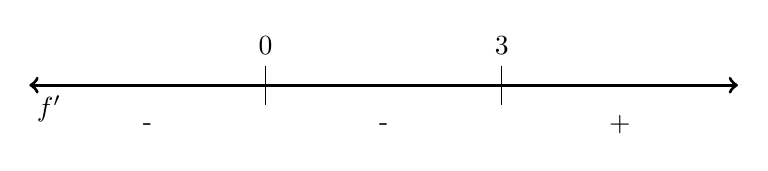
\begin{tikzpicture}
                \draw[<->, very thick] (-4.5,0) -- (4.5,0); %number line
                \draw (-1.5,0.25) -- (-1.5,-0.25); %Vertical tick marks
                \draw (1.5,0.25) -- (1.5,-0.25);
                \node () at (-4.25,-0.3) {$f'$}; %Labels
                \node () at (-1.5,0.5) {0};
                \node () at (1.5,0.5) {3};
                \node () at (-3,-0.5) {-}; %Sign markings
                \node () at (0,-0.5) {-};
                \node () at (3,-0.5) {+};
            \end{tikzpicture}
        \end{center}

        \nonindent Since the derivative changes sign only at $x=3$,\\

        \begin{center}
            \begin{tabular}{cc}
                if $x<3$ & $f'(x)\leq 0$ and $f$ is decreasing \\
                If $x>3$ & $f'(x)> 0$ and $f$ is increasing
            \end{tabular}
        \end{center}


    \subsection{Extrema, Concavity, and Inflection Points}
        The curve of $y=f(x)$ has a \textbf{local/relative maximum} at a point where $x=c$ if
        $f(c)\geq f(x)$ for all $x$ in the immediate neighborhood of $c$. If a curve has a
        relative maximum at $x=c$, then the curve changes from increasing to decreasing as $x$
        increases through $c$. \\

        \noindent The curve of $y=f(x)$ has a \textbf{local/relative minimum} at a point where
        $x=c$ if $f(c)\leq f(x)$ for all $x$ in the immediate neighborhood of $c$.
        If a curve has a relative minimum at $x=c$, then the curve changes from decreasing to
        increasing as $x$ increases through $c$. \\

        \noindent If a function is differentiable on $[a,b]$ and has a relative extremum at $
        x=c, a<c<b$, then $f'(c)=0$. \\

        \noindent The \textbf{global/absolute maximum} of a function on $[a,b]$ occurs at $x=c$
        if $f(c)\geq f(x)$ for all $x$ on $[a,b]$. The \textbf{global/absolute minimum} of a
        function on $[a,b]$ occurs at $x=c$ if $f(c)\leq f(x)$ for all $x$ on $[a,b]$. \\

        \noindent A curve is \textbf{concave upward} on an interval $(a,b)$ if the curve lies
        above the tangent lines at each point in the interval $(a,b)$. A curve is
        \textbf{concave downward} on an interval $(a,b)$ if the curve lies below the tangent
        lines at each point in the interval $(a,b)$. \\

        % @TODO: Last tikzpicture won't load need to fix
        \begin{center}
            \begin{tabular}{|c|c|}
                \hline
                $f"(x) > 0$ & Concave Up \\
                \hline
                $f"(x) < 0$ & Concave Down \\
                \hline
            \end{tabular}

            \begin{tabular}{cc}
                \begin{tikzpicture} [scale = 0.75]
                    \begin{axis}[
                        axis lines = center,
                        xmin = -7,
                        xmax = 15,
                        ymin = 0,
                        ymax = 20
                    ]
                    \addplot[
                        color = red,
                        samples = 100,
                        domain = -7:15
                    ]
                    {((x-4)^2)/(4)+2};
                    \addplot[
                        dashed,
                        color = blue,
                        domain = -1.8:1.8,
                        samples = 2
                    ]
                    {-2*x+6};
                    \addplot[
                        dashed,
                        color = blue,
                        domain = 2.2:5.8,
                        samples = 2
                    ]
                    {2};
                    \addplot[
                        dashed,
                        color = blue,
                        domain = 6.2:9.8,
                        samples = 2
                    ]
                    {2*x-10};
                    \end{axis}
                \end{tikzpicture}
                &
                \begin{tikzpicture} [scale=0.75]
                    \begin{axis}[
                        axis lines = center,
                        xmin = -7,
                        xmax = 15,
                        ymin = 0,
                        ymax = 20
                    ]
                    \addplot[
                        color = red,
                        samples = 100,
                        domain = -7:15
                    ]
                    {((x-4)^2)/(-4)+18};
                    \addplot[
                        dashed,
                        color = blue,
                        domain = -3.8:-0.2,
                        samples = 2
                    ]
                    {3*x+15};
                    \addplot[
                        dashed,
                        color = blue,
                        domain = 2.2:5.8,
                        samples = 2
                    ]
                    {18};
                    \addplot[
                        dashed,
                        color = blue,
                        domain = 8.2:11.8,
                        samples = 2
                    ]
                    {-3*x+39};
                    \end{axis}
                \end{tikzpicture}
            \end{tabular}
        \end{center}



    \subsection{Related Rates}
        Related rates are an application of implicit differentiation that allow us to solve for
        rates of change and other quantities in an applied real-world system, typically growing
        with respect to time. \\

        \noindent \color{blue} \colorit{Example 1: Air is being pumped into a spherical balloon at
        a rate of 5 $\text{cm}^3$/min. Determine the rate at which the radius of the balloon is
        increasing when the diameter of the balloon is 20 cm.} \color{black} \\

        \noindent We are given $\frac{dV}{dt}=5$ and we want to find $\frac{dr}{dt}_{r=10}$. \\
        \noindent Assuming the balloon is perfectly spherical, its volume is given by
        $V=\frac{4}{3}\pi r^3$. Then

        \begin{align*}
            \frac{dV}{dt}        &= 4\pi r^2 \frac{dr}{dt} \\
            5                    &= 4\pi (10)^2 \frac{dr}{dt} \\
            \frac{dr}{dt}_{r=10} &= \frac{1}{80\pi} \text{cm/min}
        \end{align*}

        \noindent \color{blue} \textit{Example 2: A 15 foot ladder is resting against the wall.
        The bottom is initially 10 feet away from the wall and is being pushed towards the wall at
        the rate of $\frac{1}{4}$ ft/sec. How fast is the top of the ladder moving 12 seconds
        after we start pushing?} \color{black} \\

        \noindent Let us first sketch the situation: \\

        \begin{figure}[hbt!]
            \centering
            \includegraphics[scale=0.6]{Resources/Unit3DiffferentiationApps/Related_Rates_1}
        \end{figure}

        \noindent Let the vertical distance between the ground and the ladder be represented by $y$,
        the horizontal distance between the wall and the end of the ladder be represented by $x$,
        and let the length of the ladder be represented by $c=15$. Then from the Pythagorean Theorem,

        \begin{align*}
            x^2 + y^2       &= c^2 = 15 \\
            2xx' + 2yy'     &= 0 \\
            yy'             &= -xx' \\
            \frac{dy}{dt}   &= \frac{-x\cdot\frac{dx}{dt}}{y} \\
            \frac{dy}{dt}   &= \frac{-7(-\frac{1}{4})}{\sqrt{176}} \\
            \frac{dy}{dt}   &= \frac{7}{4\sqrt{1176}} \approx 0.1319 \text{ft/sec}
        \end{align*}

        Notice that we were able to obtain exact values for $x$ and $y$ because
        $x=10+tx'=10-\frac{1}{4}(12) = 7$ and

        \begin{align*}
            x^2+y^2     &=c^2 \\
            49 + y^2    &= 225 \\
            y           &= \sqrt{176}
        \end{align*}

        \noindent \color{blue} \textit{Example 3: Suppose that we have two resistors connected in
        parallel with resistances $R_1$ and $R_2$ measured in $\Omega$. The total resistance $R$
        is then given by}

        \begin{equation*}
            \frac{1}{R} = \frac{1}{R_1} + \frac{1}{R_2}
        \end{equation*}

        \noindent Suppose that $R_1$ is increasing at a rate of 0.4 $\Omega$/min and $R_2$ is
        decreasing at a rate of 0.7 $\Omega$/min. At what rate is $R$ changing when $R_1=80\Omega$
        and $R_2=105\Omega$? \color{black} \\

        \noindent When $R_1=80\Omega$ and $R_2=105\Omega$,

        \begin{align*}
            \frac{1}{R}     &= \frac{1}{80} + \frac{1}{105} \\
            \frac{1}{R}     &= \frac{37}{1680} \\
            R               &= \frac{1680}{37}
        \end{align*}

        \noindent Then

        \begin{align*}
            \frac{1}{R}     &= \frac{1}{R_1} + \frac{1}{R_2} \\
            -\frac{R'}{R^2} &= -\frac{R'_1}{(R_1)^2} - \frac{R'_2}{(R_2)^2} \\
            \frac{dR}{dt}   &= R^2\left(\frac{R'_1}{(R_1)^2}+\frac{R'_2}{(R_2)^2}\right) \\
            \frac{dR}{dt}   &= \left(\frac{1680}{37}\right)\left(\frac{0.4}{80^2}-\frac{0.7}{105^2}\right) \\
            \frac{dR}{dt}   &\approx -0.002045 \Omega\text{/min}
        \end{align*}


    \subsection{Tangent-Line Approximations}
        Given a function $f(x)$ that is differentiable at $x=a$, we know that the slope of the
        tangent line to $f(x)$ at $(a,f(a))$ is $f'(a)$. Thus, the tangent line $L(x)$ through
        $(a,f(a))$ with slope $f'(a)$ has an equation in point-slope form given by

        \begin{equation*}
            L(x) = f(a) + f'(a)(x-a)
        \end{equation*}

        \noindent Below is a graph of the function $y=f(x)$ and its linearization $y=L(x)$.

        \begin{figure}[hbt!]
            \centering
            \includegraphics[scale=0.6]{Resources/Unit3DiffferentiationApps/Linearization}
        \end{figure}

        \pagebreak
        \noindent \color{blue} \textit{Example 1: Determine the linear approximation for
        $f(x)=\sqrt[3]{x}$ at $x=8$. Use the linear approximation to approximate the value of
        $\sqrt[3]{8.05}$} and $\sqrt[3]{25}$. \color{black}

        \begin{align*}
            L(x)        &= f(8) + f'(8)(x-8) \\
            &= 2 + \frac{1}{3}8^{-\frac{2}{3}}(x-8) \\
            &= \frac{1}{12}x + \frac{4}{3} \\
            L(8.05)     &\approx 2.0041667 \\
            L(25)       &\approx 3.4166667
        \end{align*}



    \subsection{The Newton-Raphson Method}
        The \textbf{Newton-Raphson Method} is a way to quickly find an \textit{approximation}
        iteratively for the root of a real-valued function $f(x)=0$. It is founded on the concept
        that a continuous and differentiable function can be approximated by a tangent line to it. \\

        \noindent Suppose you want to find the root of a continuous, differentiable function $f(x)$ and you
        know that the target root is near the point $x_0$. Then with Newton's Method, an approximation
        for the root $x_1$ is given by

        \begin{equation*}
            x_1 = x_0 - \frac{f(x_0)}{f'(x_0)}
        \end{equation*}

        \noindent This method can be repeated as many times as necessary to get the desired accuracy.
        Then the generalization of Newton's Method is given by \\

        \begin{equation*}
            x_{n+1}     = x_n - \frac{f(x_n)}{f'(x_n)}
        \end{equation*}

        \noindent Below is a visual demonstration of Newton's Method.

        \begin{figure}
            \centering
            \includegraphics{Resources/Unit3DifferentiationApps/NewtonsMethod}
        \end{figure}

        \noindent \color{blue} \textit{Example: Find the root of the equation $x^2-4x-7=0$ near
        $x=5$}. \color{black} \\

        \noindent We are given $x_0=5$. Let $f(x)=x^2-4x-7$ and $f'(x)=2x-4$. Then,

        \begin{align*}
            x_1 &= 5 - \frac{5^2-4\cdot5-7}{2\cdot5-4} = 5-\left(\frac{-2}{6}\right)=\frac{16}{3}
            \approx 5.33333 \\
            x_2 &= \frac{16}{3} - \frac{\left(\frac{16}{3}\right)^2-4\left(\frac{16}{3}\right)-7}
            {2\left(\frac{16}{3}\right)-4} = \frac{16}{3}-\frac{\frac{1}{9}}{\frac{20}{3}}
            = \frac{16}{3} - \frac{1}{60} = \frac{319}{60} \approx 5.31667 \\
            x_3 &= \frac{319}{60} - \frac{\left(\frac{319}{60}\right)^2-4\left(\frac{319}{60}\right)-7}
            {2\left(\frac{319}{60}\right)-4} = \frac{319}{60} -
            \frac{\frac{1}{3600}}{\frac{398}{60}} \approx 5.31662
        \end{align*}


    \subsection{Optimization}
        \textbf{Optimization} uses a function's derivatives to find the maximum or
        minimum value of that function. \\

        \noindent \color{blue} \textit{Example 1: We need to enclose a rectangular field with a
        fence. We have 500 feet of fencing material and a building is on one side of the field
        and so won't need any fencing. Determine the dimensions of the field that will enclose the
        largest area.} \color{black} \\

        \noindent Let us first visualize the situation:

        \begin{figure}
            \centering
            \includegraphics[scale=0.4]{Resources/Unit3DifferentiationApps_optimization}
        \end{figure}

        \noindent We want to maximize the area of the field and we only have 500 ft of fencing
        material. So, we represent this system by the following equations:

        \begin{align*}
            \text{Maximize: } A     &= xy \\
            \text{Constraint: } 500 &= x + 2y
        \end{align*}

        \noindent Solving the constraint equation for $x$, we get $x=500-2y$. We can substitute this
        into the area function, giving us \\

        \begin{align*}
            A(y)  &= (500-2y)y \\
            &= 500y-2y^2 \\
            A'(y) &= 500-4y \\
            0     &= 500 - 4y \\
            y     &= 125 \\
            x     &= 500-2(125) = 250
        \end{align*}

        \noindent Thus, the dimensions of the field that wil give the largest area are 250 x 125. \\

        \noindent \color{blue} \textit{Example 2: A manufacturer needs to make a cylinderical can
        that will hold 1.5 litres of liquid. Determine the dimensions of the can that will
        minimize the amount of material used in its constraint.} \color{black} \\

        \noindent We will eventually need the radius and height of the can in terms of a linear
        measurement unit, instead of litres. Thus, the volume, 1.5 litres, becomes 1500 $\text{cm}^3$.

        \begin{align*}
            \text{Minimize:} A      &= 2\pi rh+2\pi r^2 \\
            \text{Constraint:} 1500 &= \pi r^2 h \\
            h                       &= \frac{1500}{\pi r^2} \\
            \implies A(r)           &= 2\pi r\left(\frac{1500}{\pi r^2}\right) + 2\pi r^2 \\
            A(r)                    &= 2\pi r^2 + \frac{3000}{r} \\
            A'(r)                   &= 4\pi r - \frac{3000}{r^2} \\
            A'(r)                   &= \frac{4\pi r^3 - 3000}{r^2} \\
            0                       &= \frac{4\pi r^3 - 3000}{r^2} \\
            r                       &= \sqrt[3]{\frac{750}{\pi}} \\
            r                       &= 6.2035 \\
            h                       &= \frac{1500}{\pi(6.2035)^2} \\
            h                       &= 12.4070
        \end{align*}

        \noindent Thus, the dimensions of the can that will minimize the material required to
        construct the box are a radius of 6.2035 cm and a height of 12.4070 cm.